\section*{Introduzione}

Nel seguente documento verranno descritte ed illustrate le fasi di sviluppo del progetto \textbf{Zillow Prize: Zillow’s Home Value Prediction (Zestimate)}.
Nello specifico saranno evidenziate e spiegate le decisioni prese, che hanno portato al completamento dello stesso.
Saranno utilizzati diversi grafici per mostrare alcuni dei dati importanti che hanno portato alle decisioni finali prese.

\section*{Creazione del dataframe}
Inizialmente è stato fatto l'import delle diverse librerie e moduli che sono stati utilizzati all'interno del progetto.
Successivamente sono stati caricati i dataset e trasformati in data frame con l'utilizzo della libreria Pandas. Sempre grazie a tale libreria è stato poi fatta 
l'unione tra i due dataset contenenti diverse feature utili, quali ``\textbf{logerror}'' (la variabile risposta) o la ``\textbf{transactiondate}'' (data acquisto), così da avere tutte 
le istanze all'interno di un unico data frame.

\section*{Pulizia dei dati}
Stampando il contenuto e il tipo delle varie feature contenute nel data frame appena costruito, è risultato che per la maggior parte erano di tipo \textbf{float64} mentre solo alcune erano di tipo \textbf{object}. 
Le prime non presentavano problemi nella gestione, mentre per quanto riguarda le seconde è stato necessario effettuare altre operazioni che saranno illustrate successivamente. 
Inizialmente abbiamo cercato di gestire subito la feature ``\textbf{transactiondate}'' andando a crearne di nuove, come la '\textbf{builded\_buyed}' che mantiene un conteggio dei giorni trascorsi dal giorno in cui è stata effettuata la vendita della casa all'anno in cui è stata effettivamente
costruita (l'anno di costruzione viene considerato completo per ogni casa, quindi 365 giorni).\\
Questa nuova feature ci ha consentito di andare poi a rimuovere le istanze con ``\textbf{parcelid}'' duplicati, ossia id assegnati a più vendite della stessa abitazione. Ci siamo interessati nel mantenere le case con il valore più alto della feature ``\textbf{builded\_buyed}'', in quanto corrispondenti alla 
transazione più recente. Abbiamo pensato che transazioni più recenti avrebbero fatto riferimento a valori complessivi della casa più attuali.\\
Per la pulizia dei dati abbiamo deciso di cancellare tutte le feature che avevano un missing rate maggiore del \textbf{50\%}. Per quanto riguarda invece le feature con una percentuale inferire al \textbf{50\%} abbiamo deciso di correggere i valori mancanti con la media, nel caso di variabili numeriche, oppure con la mediana per variabili di tipo categoriale.
Questo processo è stato effettuato nelle fasi più avanzate del progetto, ossia dopo l'aggiunta di eventuali nuove variabili.

\section*{Featrue engeneering}
In quanto ad aggiunta di nuove feature, abbiamo deciso di inserirne alcune sulla base di quelle preesistenti all'interno del dataset e di gestirne alcune con maggiore attenzione.
Inizialmente siamo andati a sistemare due feature, rispettivamente ``\textbf{house\_dim}'' e ``\textbf{censustractandblock}''. Lo scopo di queste due featrue è quello di recuperare i valori mancanti da altre presenti nel dataset. In entrambi i casi avevamo notato che potevano essere recuperati tali valori da altre feature molto simili se non identiche.\\
Successivamente abbiamo aggiunto due nuove feature binarie ``\textbf{missed\_room}'' e ``\textbf{pre\_house\_dim}''. Il loro scopo è quello di mantenere informazioni riguardo alla mancanza di dati per quanto riguarda la presenza dei garage oppure la dimensione totale della casa, prima che tale informazione sia rimossa dal dataframe oppure gestita.\\
Abbiamo poi deciso di gestire quelle che erano le tre feature 'problematiche' di tipo \textbf{object} già citate in precedenza. Per esse abbiamo utilizzato l'algoritmo \textbf{LabelEncoder()} così da poter associare ad ogni singolo elemento unico un id numerico, facilmente gestibile dai nostri futuri modelli. Non abbiamo potuto utilizzare \textbf{OneHotEncoder()}
in quanto tutte e tre le feature possedevano un numero molto elevato di valori unici, andando anche a selezionare solamente quelli più frequenti.\\
Nell'ultima fase di questa sezione abbiamo poi creato alcune nuove feature.
La prima feature creata è quella inerente ai beni di lusso. Il suo scopo è quello di mantenere un punteggio sulla base della presenza di alcune determinati oggetti che abbiamo considerato di lusso, quali la SPA, la piscina, il condizionatore oppure il camino.
La seconda feature creata è la '\textbf{ValueProperty}' il cui scopo è quello di stimare il valore dell'abitazione in base alle tasse applicate.\\ 
Abbiamo aggiunto poi una serie di feature che mantengono informazioni inerenti alla media di altre variabili. Nello specifico ``\textbf{avg\_valuexzip}'' e ``\textbf{avg\_taxzip}'' che memorizzano il valore medio stimato della casa e il valore medio delle tasse sulla base dello zipcode associato ad una casa. Le seconde due create invece sono 
``\textbf{avg\_day}'' e ``\textbf{avg\_month}'' che prendono in considerazione il ``\textbf{logerror}'' medio in base al giorno d'acquisto (all'interno di un mese) oppure al mese d'acquisto (all'interno di un anno).\\
Infine, l'ultima feature aggiunta è ``\textbf{room\_count}'' che mantiene un punteggio in base alla stima del numero di stanze presenti in una casa e la dimensione di tali.\\
Dopo aver rimosso eventuali feature non più utili e quindi non necessarie da passare ai modelli, abbiamo deciso di affidaci all'algoritmo \textbf{RFECV} che allenando dei modelli di \textbf{Random forest}, ci ha selezionato quelle che erano le feature più importanti, ossia che avrebbero fornito un contributo maggiore nelle predizioni finali che saremmo andati ad effettuare.
\begin{figure}[h]
    \centerline{\frame{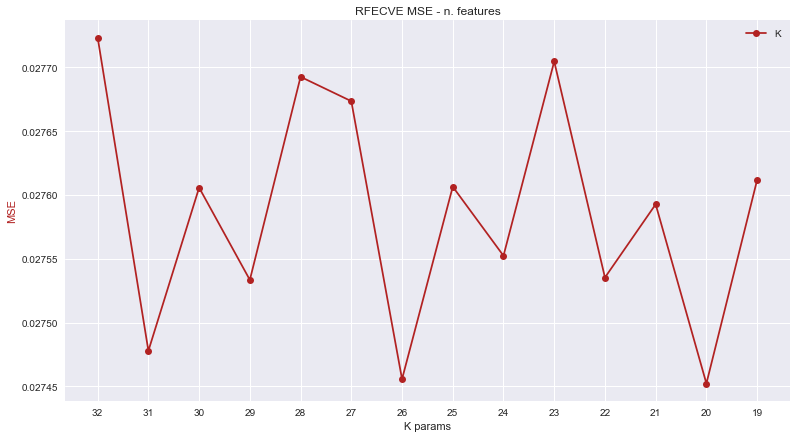
\includegraphics[scale=.45]{images/RFECVK.png}}}
   \caption{Grafico dei risultati ottenuto con \textbf{RFECV}. \textbf{MSE} al variare delle feature selezionate}
\end{figure}

\section*{Analisi dataframe post lavorazione dati}
Terminata la fase di pulizia dei dati e la selezione delle feature, abbiamo effettuato la divisione in train e test dei dati ed abbiamo verificato come fossero distribuiti i dati della variabile risposta, ossia il ``\textbf{logerror}''.
Dalla piccola analisi effettuata è risultato che la distribuzione era molto simile a quella di una normale, a parte per la presenza di alcuni valori anomali. Effettuando varie prove e rimuovendo infine tali valori dal train set abbiamo ottenuto 
valori migliori nelle predizioni finali, decidendo quindi di mantenere le modifiche apportate.

\section*{Creazione modelli di regressione e confronti}
Come modelli di Regressione abbiamo deciso di utilizzare i seguenti : \textbf{Random forest}, \textbf{Regressione lineare}, \textbf{Knn}, \textbf{SVR} e \textbf{AdaBoost}.
Per allenare i diversi modelli abbiamo deciso di utilizzare la funzione \textbf{GridSearchCV}, così da effettuare prima un tuning dei possibili parametri da utilizzare per ogni singolo modello e rilevare quelli migliori effettuando predizioni nei validation set.
Abbiamo poi utilizzato i risultati ottenuti per andare ad allenare il modelli con i migliori parametri rilevati, ed effettuare così le predizioni finali sul test. Le statistiche ottenute sono poi state inserite in una tabella e confrontate.
\begin{figure}[htbp]
    \centerline{\frame{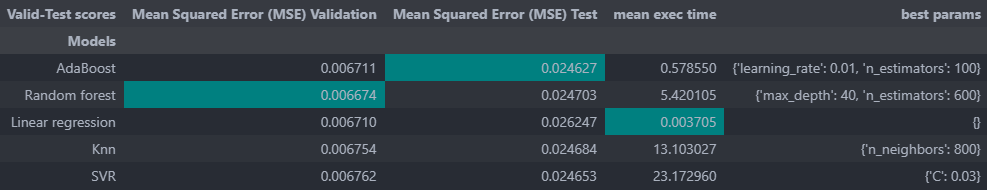
\includegraphics[scale=.5]{images/stats.png}}}
   \caption{Tabella dei risultati finali ottenuti da ogni modello}
\end{figure}
\\La metrica per misurare l'accuratezza di un modello che abbiamo deciso di impiegare è lo \textbf{Mean Squared error}. Per ogni modello abbiamo mostrato quindi l'\textbf{MSE} ottenuto prima sul validation set e poi sul test set, il tempo medio d'esecuzione impiegato e i parametri che sono risultati essere i migliori per esso.
Com'è facilmente notabile, il modello che ha offerto il più basso \textbf{MSE} sul test set è stato \textbf{AdaBoost}. Conseguentemente abbiamo deciso di utilizzarlo come riferimento per verificare quali fossero le istanze con un errore di predizione maggiore.

\section*{Analisi degli errori e conclusioni}
In quest'ultima fase abbiamo quindi analizzato gli errori ottenuti nella predizione col modello migliore tra quelli testati.
Inizialmente abbiamo provato a stamparci diversi scatterplot per vedere quale mostrasse maggiormente un pattern comune su cui il modello avesse più difficoltà nell'effettuare le predizioni, portandolo quindi a sbagliare. 
Tra tutti i grafici abbiamo notato che quello per la feature ``\textbf{propertyzoningdesc}'' mostra in due differenti distretti un particolare accumulo di errori più gravi rispetto alla media.
\begin{figure}[htbp]
    \centerline{\frame{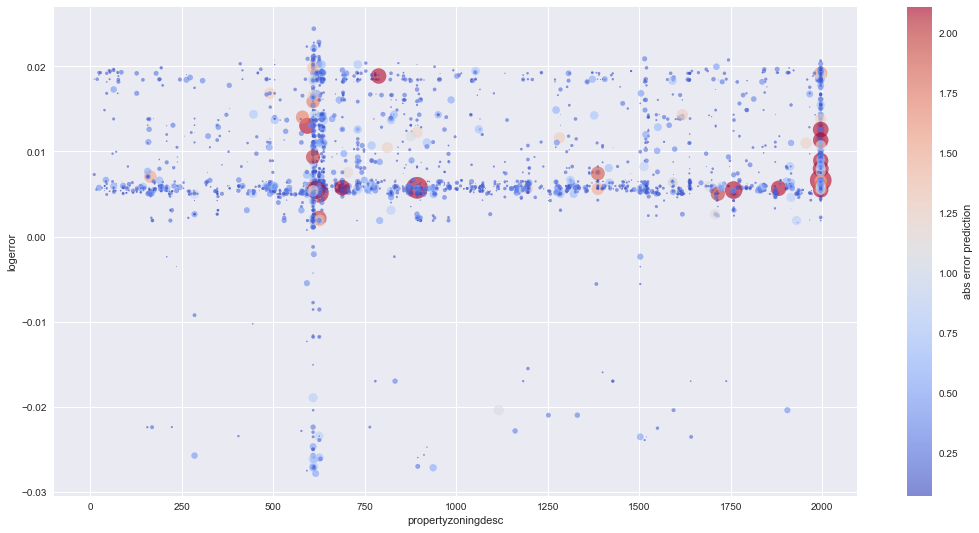
\includegraphics[scale=.37]{images/errors1.png}}}
   \caption{Scatterplot degli errori di predizione. La dimensione ed il colore di un punto identificano la quantità di errore nella predizione.}
\end{figure}
\\
Nello specifico i due distretti maggiormente affetti da errori di predizione, com'è visibile anche nel grafico sottostante, sono quelli associati all'id ``\textbf{1996}'' e nel range ``\textbf{600 - 691}''. Stampando tali istanze in un file csv, abbiamo notato che uno dei principali motivi che abbia portato ad 
un alto errore sopratutto in quelle zone è la presenza di molte feature affette da missing values, i cui valori sono quindi stati riempiti con la media e la mediana. Le due feature che probabilmente impattano maggiormente sull'errore di predizione sono ``\textbf{builded\_buyed}'' (giorni passati tra ano costruzione e data ultimo acquisto) e 
``\textbf{structuretaxvaluedollarcnt}'', in quanto risultavano tra le più importanti per effettuare le predizioni. Un'altro fattore interessante che può aver portato i modelli a commettere tali errori è dato dalla presenza di alcune istanze avanti valori anomali delle tasse sull'abitazione, ossia abitazioni aventi alti valori di tasse da dover 
pagare, nonostante le dimensioni contenute della casa. Questo potrebbe essere comunque dovuto alla zona d'appartenenza dell'abitazione, tuttavia è comunque una situazione che pensiamo sia giusto segnalare.\\
Infine, un'ultima particolarità che abbiamo notato, anche per quanto riguarda le istanze ben predette dal modello, è la tendenza ad effettuare la maggior parte degli errori soprattutto nelle istanze positive del ``\textbf{logerror}''. Nel grafico abbiamo escluso le istanze affette da poco errore, tuttavia controllando anche nel file csv era facilmente 
notabile come le istanze predette con un ridotto tasso d'errore erano tutte quelle associate ad un valore positivo di tale feature.\\
Nel complesso possiamo quindi ritenerci soddisfatti dei risultati ottenuti e dell'esperienza fatta.